% =============================================================================
% Presentación para el video – INFB8091 Desempeño de Sistemas (UTEM, 2026-2)
% Guion: guía, sección 7.3 (resumido). Duración objetivo: 8–10 minutos.
% La esquina inferior derecha de cada diapositiva queda libre para la ventana
% de la cámara de quien presenta (requisito del enunciado).
%
% Compilar desde esta carpeta:  latexmk -pdf presentacion.tex
% =============================================================================
\documentclass[aspectratio=169,11pt]{beamer}

\usepackage[utf8]{inputenc}
\usepackage[T1]{fontenc}
\usepackage[spanish,es-nodecimaldot]{babel}
\usepackage{lmodern}
\usepackage{booktabs}
\usepackage{tikz}
\usetikzlibrary{positioning,fit,arrows.meta}

\graphicspath{{../informe/}{../carga/graficos/}{../Capturas configuracion/}}

% --- Identidad UTEM (colores del logo) ---------------------------------------
\definecolor{azulutem}{RGB}{0,78,170}
\definecolor{verdeutem}{RGB}{120,191,38}
\definecolor{grisutem}{RGB}{82,81,78}
\usefonttheme{professionalfonts}
\setbeamertemplate{navigation symbols}{}
\setbeamercolor{frametitle}{fg=azulutem}
\setbeamercolor{title}{fg=azulutem}
\setbeamercolor{structure}{fg=azulutem}
\setbeamercolor{normal text}{fg=black}
\setbeamerfont{frametitle}{series=\bfseries,size=\Large}
\setbeamertemplate{itemize item}{\color{verdeutem}$\blacksquare$}
\setbeamertemplate{itemize subitem}{\color{azulutem}--}
\setbeamertemplate{frametitle}{%
  \vspace{0.35cm}\hspace{0.1cm}\insertframetitle\hfill
  \raisebox{-0.15cm}{
\includegraphics[height=0.75cm]{logo-utem.png}}\hspace{0.2cm}\par
  \vspace{-0.1cm}{\color{verdeutem}\rule{\paperwidth}{1.5pt}}}
% Pie a la izquierda: la derecha queda libre para la cámara.
\setbeamertemplate{footline}{%
  \hspace{0.3cm}\color{grisutem}\scriptsize Subligol · INFB8091 Desempeño de Sistemas · \insertframenumber\vspace{0.25cm}}

% Texto que llega al borde inferior: se limita al 64 % del ancho (cámara a la derecha).
\newcommand{\izq}[1]{\begin{minipage}[t]{0.64\textwidth}#1\end{minipage}}
\newcommand{\dato}[2]{\begin{tabular}{@{}c@{}}{\Large\bfseries\color{azulutem}#1}\\[-1pt]{\scriptsize\color{grisutem}#2}\end{tabular}}

\begin{document}

% -----------------------------------------------------------------------------
\begin{frame}[plain]
  \begin{center}
    
\includegraphics[height=1.9cm]{logo-utem.png}\\[0.3cm]
    {\color{verdeutem}\rule{0.8\paperwidth}{1.5pt}}\\[0.5cm]
    {\LARGE\bfseries\color{azulutem} Desempeño de Subligol bajo carga}\\[0.2cm]
    {\large Un comercio electrónico medido con GA4, k6 y Prometheus}\\[0.6cm]
    {\bfseries\color{azulutem} Grupo Deadlock}\\[0.1cm]
    Wladimir Gallardo · Rodrigo Donoso · Leonardo Solís\\[0.1cm]
    {\small Profesor: Javier Aranda · INFB8091 Desempeño de Sistemas · 16 de noviembre de 2026}
  \end{center}
\end{frame}

% -----------------------------------------------------------------------------
% Bloque 1 – Grupo, comercio y objetivos
\begin{frame}{Subligol y objetivos}
  \vspace{0.6cm}
  \begin{columns}[T]
    \begin{column}{0.55\textwidth}
      \textbf{Subligol}: tienda en línea de insumos de sublimación e impresión.
      \begin{itemize}
        \item Catálogo de 500 productos con filtros y búsqueda
        \item Carrito, registro e inicio de sesión
        \item Checkout con pago simulado y Webpay (sandbox de Transbank)
        \item Home, listado y detalle con distinta carga de datos
      \end{itemize}
    \end{column}
    \begin{column}{0.40\textwidth}
      \textbf{Objetivos}
      \begin{itemize}
        \item Instrumentar con GA4
        \item Generar carga con k6
        \item Medir latencia, errores y recursos
        \item Hallar la saturación
      \end{itemize}
    \end{column}
  \end{columns}
\end{frame}

% -----------------------------------------------------------------------------
% Bloque 2 – Arquitectura y uso del agente
\begin{frame}{Arquitectura}
  \vspace{0.75cm}
  \centering
  \begin{tikzpicture}[scale=0.82, transform shape,
    caja/.style={draw=azulutem, rounded corners=3pt, align=center, minimum width=2.4cm, minimum height=0.9cm, font=\footnotesize},
    zona/.style={draw=verdeutem, dashed, rounded corners=6pt, inner sep=7pt},
    flecha/.style={-{Stealth[length=2mm]}, thick, azulutem}]
    \node[caja] (nav) {Navegador\\React + Vite};
    \node[caja, below=0.6cm of nav] (k6) {Generador k6};
    \node[caja, right=1.2cm of nav] (caddy) {Caddy\\HTTPS};
    \node[caja, right=0.8cm of caddy] (api) {API\\Node + Express};
    \node[caja, right=0.8cm of api] (db) {PostgreSQL 16};
    \node[caja, below=0.6cm of api] (prom) {Prometheus\\+ Grafana};
    \node[caja, above=0.5cm of nav] (ga) {Google Analytics 4};
    \node[caja, above=0.5cm of db] (tbk) {Webpay\\(integración)};
    \node[zona, fit=(caddy)(api)(db)(prom), label={[font=\scriptsize, text=grisutem]below:VM Azure · 2 vCPU · 7,7 GB · Docker Compose}] {};
    \draw[flecha] (nav) -- (caddy);
    \draw[flecha] (k6) -| (caddy);
    \draw[flecha] (caddy) -- (api);
    \draw[flecha] (api) -- (db);
    \draw[flecha] (prom) -- (api);
    \draw[flecha] (nav) -- (ga);
    \draw[flecha] (api) |- (tbk);
  \end{tikzpicture}

  \vspace{0.15cm}
  \raggedright\small
  \izq{\textbf{Agente:} Claude Code (Claude Opus 5.5), guiado por \texttt{AGENTS.md};
  13 prompts en 6 Prompt Cards (\texttt{PromptCard.txt}).}
\end{frame}

% -----------------------------------------------------------------------------
% Bloque 3 – Demo del sitio y GA4
\begin{frame}{Demo del sitio y eventos en GA4}
  \vspace{0.6cm}
  \begin{columns}[T]
    \begin{column}{0.48\textwidth}
      \small
      \textbf{Demo en vivo} del sitio en Azure
      \begin{enumerate}
        \item Catálogo y búsqueda
        \item Detalle $\rightarrow$ agregar al carrito
        \item Pago con Webpay (tarjeta de prueba)
        \item Eventos en DebugView
      \end{enumerate}
      \textbf{GA4 vía Tag Manager}: eventos de compra, Web Vitals y
      \texttt{escenario\_prueba}.
    \end{column}
    \begin{column}{0.36\textwidth}
      \centering
      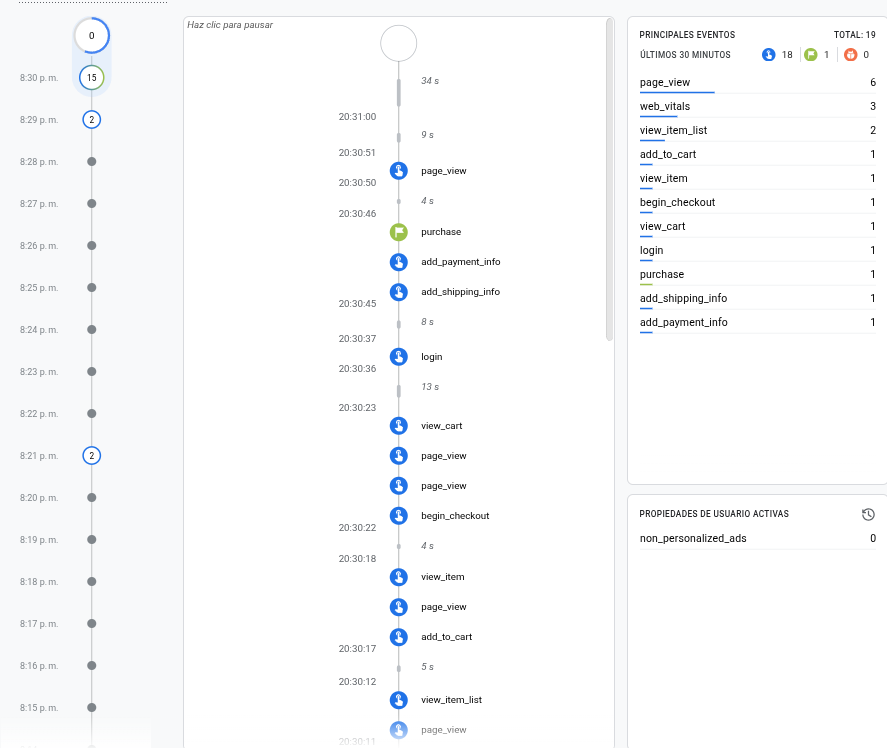
\includegraphics[height=4.3cm]{DebugView.png}
    \end{column}
  \end{columns}
\end{frame}

% -----------------------------------------------------------------------------
% Bloque 4 – Generadores de carga
\begin{frame}{Generadores de carga (k6)}
  \vspace{0.6cm}
  \begin{columns}[T]
    \begin{column}{0.42\textwidth}
      \textbf{4 perfiles de usuario}
      \begin{itemize}\small
        \item Navegante 50 \%: navega y ve detalles
        \item Buscador 25 \%: busca con filtros
        \item Abandono 15 \%: deja el carrito
        \item Comprador 10 \%: compra completa
      \end{itemize}
      \footnotesize Pausas 1--6 s · 3 repeticiones · Chrome real para Web Vitals
    \end{column}
    \begin{column}{0.53\textwidth}
      \textbf{3 escenarios}\\[0.15cm]
      \small
      \begin{tabular}{@{}ll@{}}
        \toprule
        Baja   & 5 VUs, 5 min \\
        Normal & 30 VUs, 10 min \\
        Estrés & 10 $\rightarrow$ 60 sesiones/s\\
               & mesetas de 2 min (modelo abierto) \\
        \bottomrule
      \end{tabular}\\[0.25cm]
      \textbf{SLO:} p95 $<$ 800 ms · errores $<$ 1 \%
    \end{column}
  \end{columns}
\end{frame}

% -----------------------------------------------------------------------------
% Bloque 5 – Resultados
\begin{frame}{Baja y normal: sin degradación}
  \vspace{0.6cm}
  \begin{columns}[T]
    \begin{column}{0.62\textwidth}
      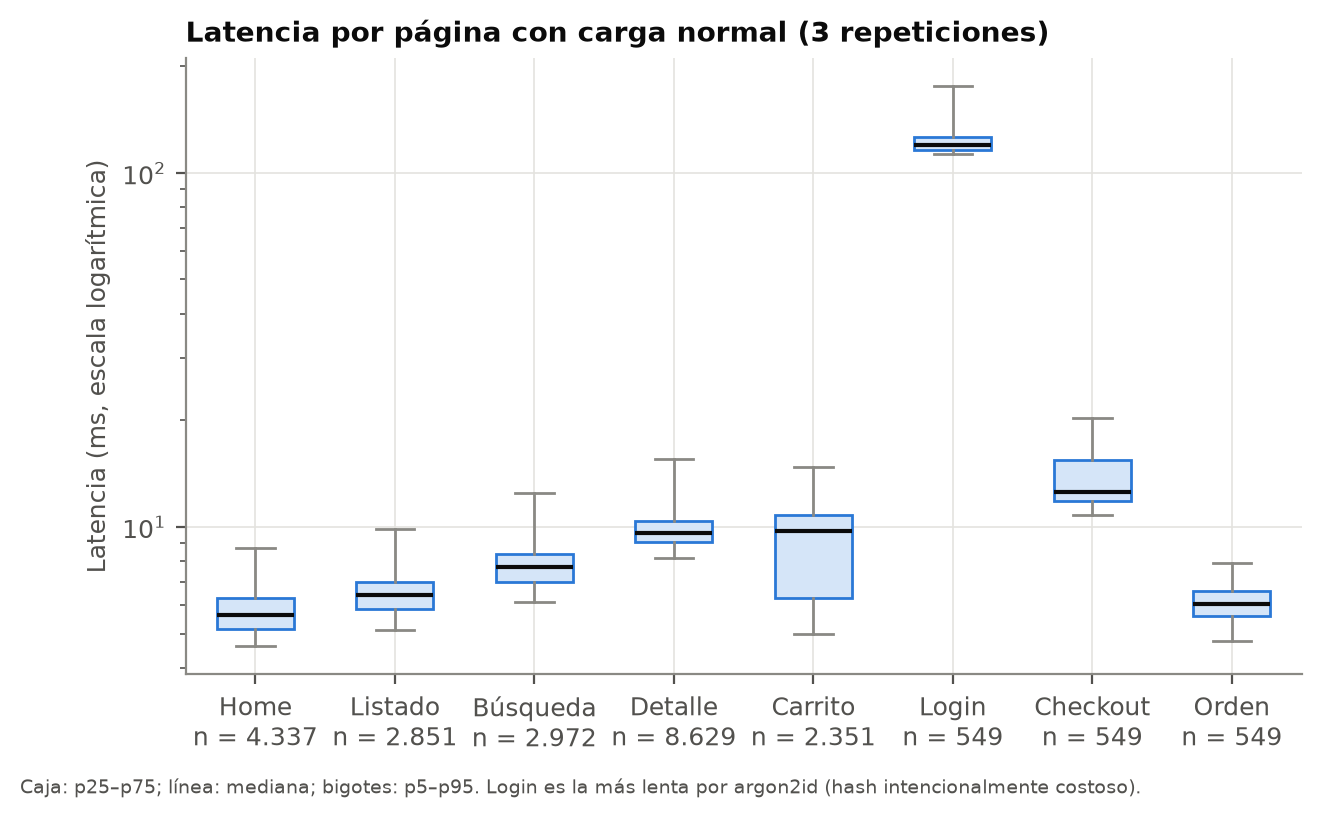
\includegraphics[width=\linewidth]{08_boxplot_paginas_normal.png}
    \end{column}
    \begin{column}{0.34\textwidth}
      \centering
      \dato{18,5 / 17,5 ms}{p95 baja / normal (6× más carga)}\\[0.3cm]
      \dato{0 \%}{errores · CPU de la VM 6 \% y 11 \%}
    \end{column}
  \end{columns}
\end{frame}

\begin{frame}{Estrés: punto de saturación}
  \vspace{0.55cm}
  \begin{columns}[T]
    \begin{column}{0.36\textwidth}
      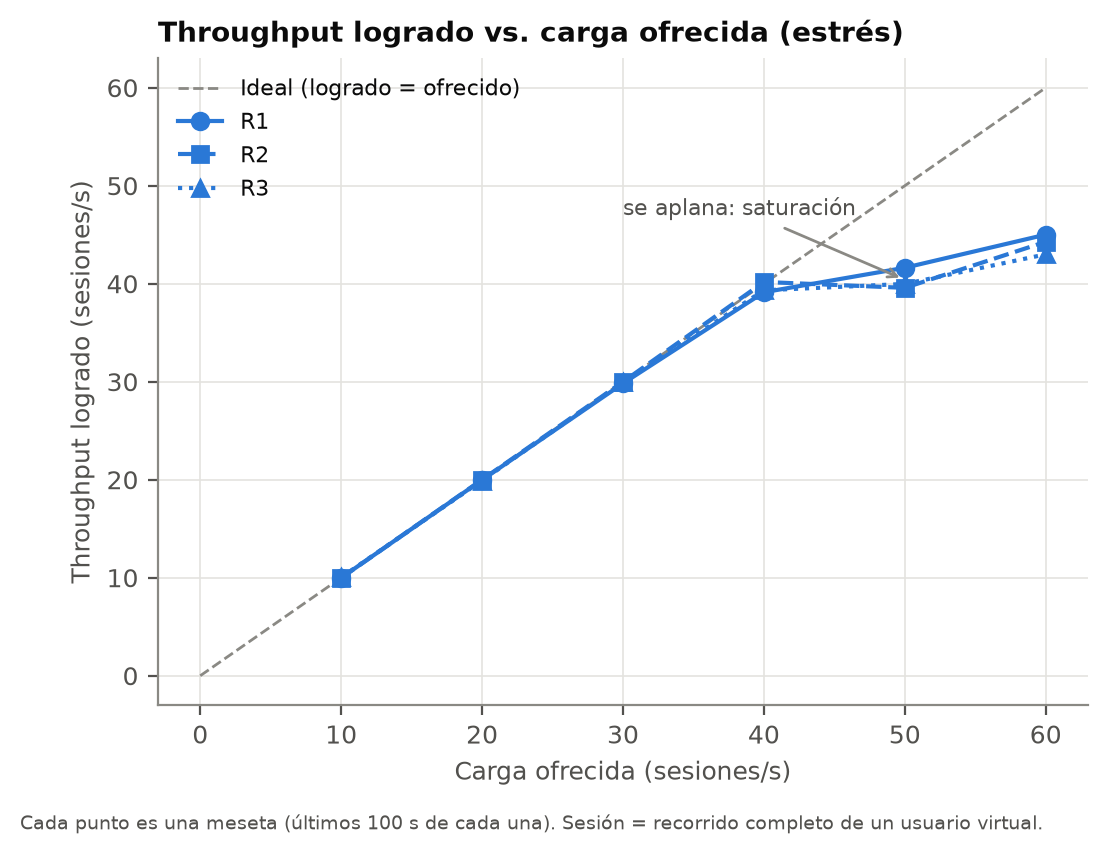
\includegraphics[width=\linewidth]{03_throughput_vs_ofrecido.png}
    \end{column}
    \begin{column}{0.36\textwidth}
      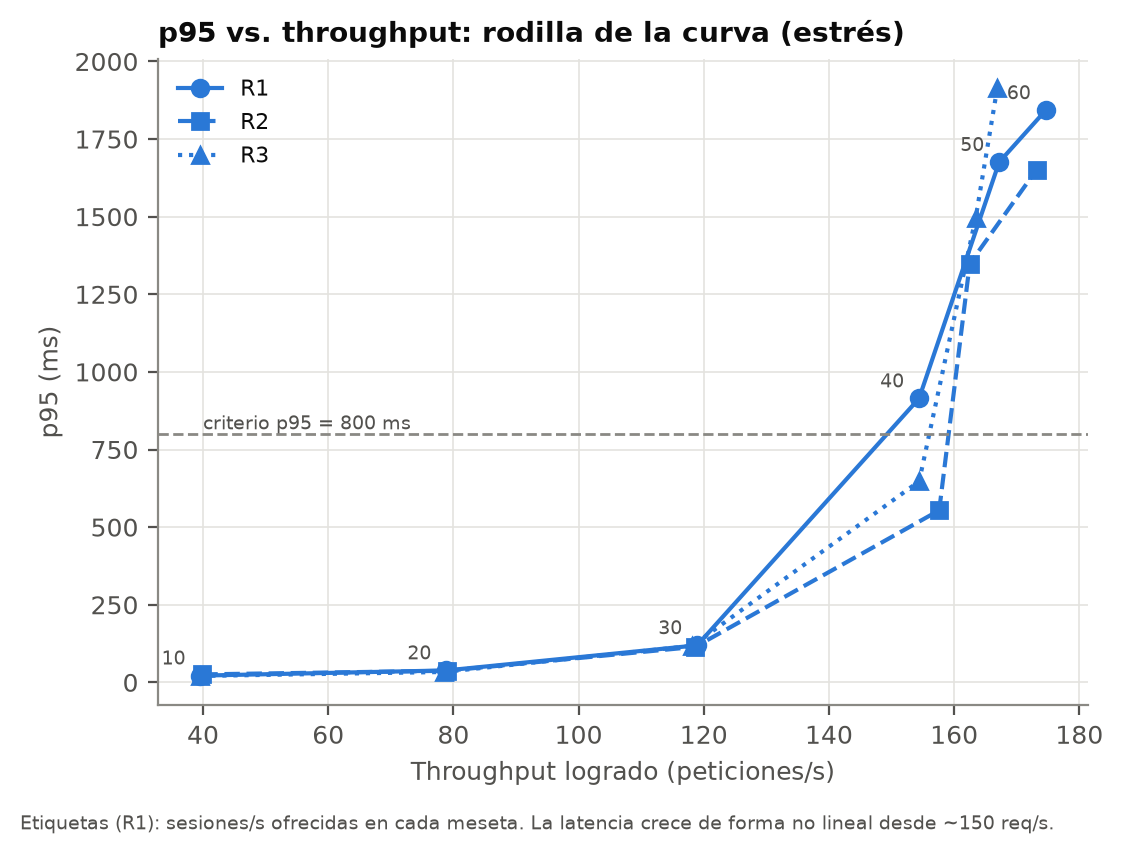
\includegraphics[width=\linewidth]{04_p95_vs_throughput.png}
    \end{column}
    \begin{column}{0.22\textwidth}\end{column}
  \end{columns}
  \vspace{0.1cm}
  \izq{\begin{itemize}\small
    \item \textbf{Rodilla: 40 ses/s ($\sim$155 req/s)}, p95 de 117 a 705 ms
    \item Saturación en \textbf{50 ses/s} · máximo \textbf{$\sim$172 req/s}
  \end{itemize}}
\end{frame}

\begin{frame}[t]{Recurso limitante: la CPU de la VM}
  \vspace{0.55cm}
  \begin{columns}[T]
    \begin{column}{0.48\textwidth}
      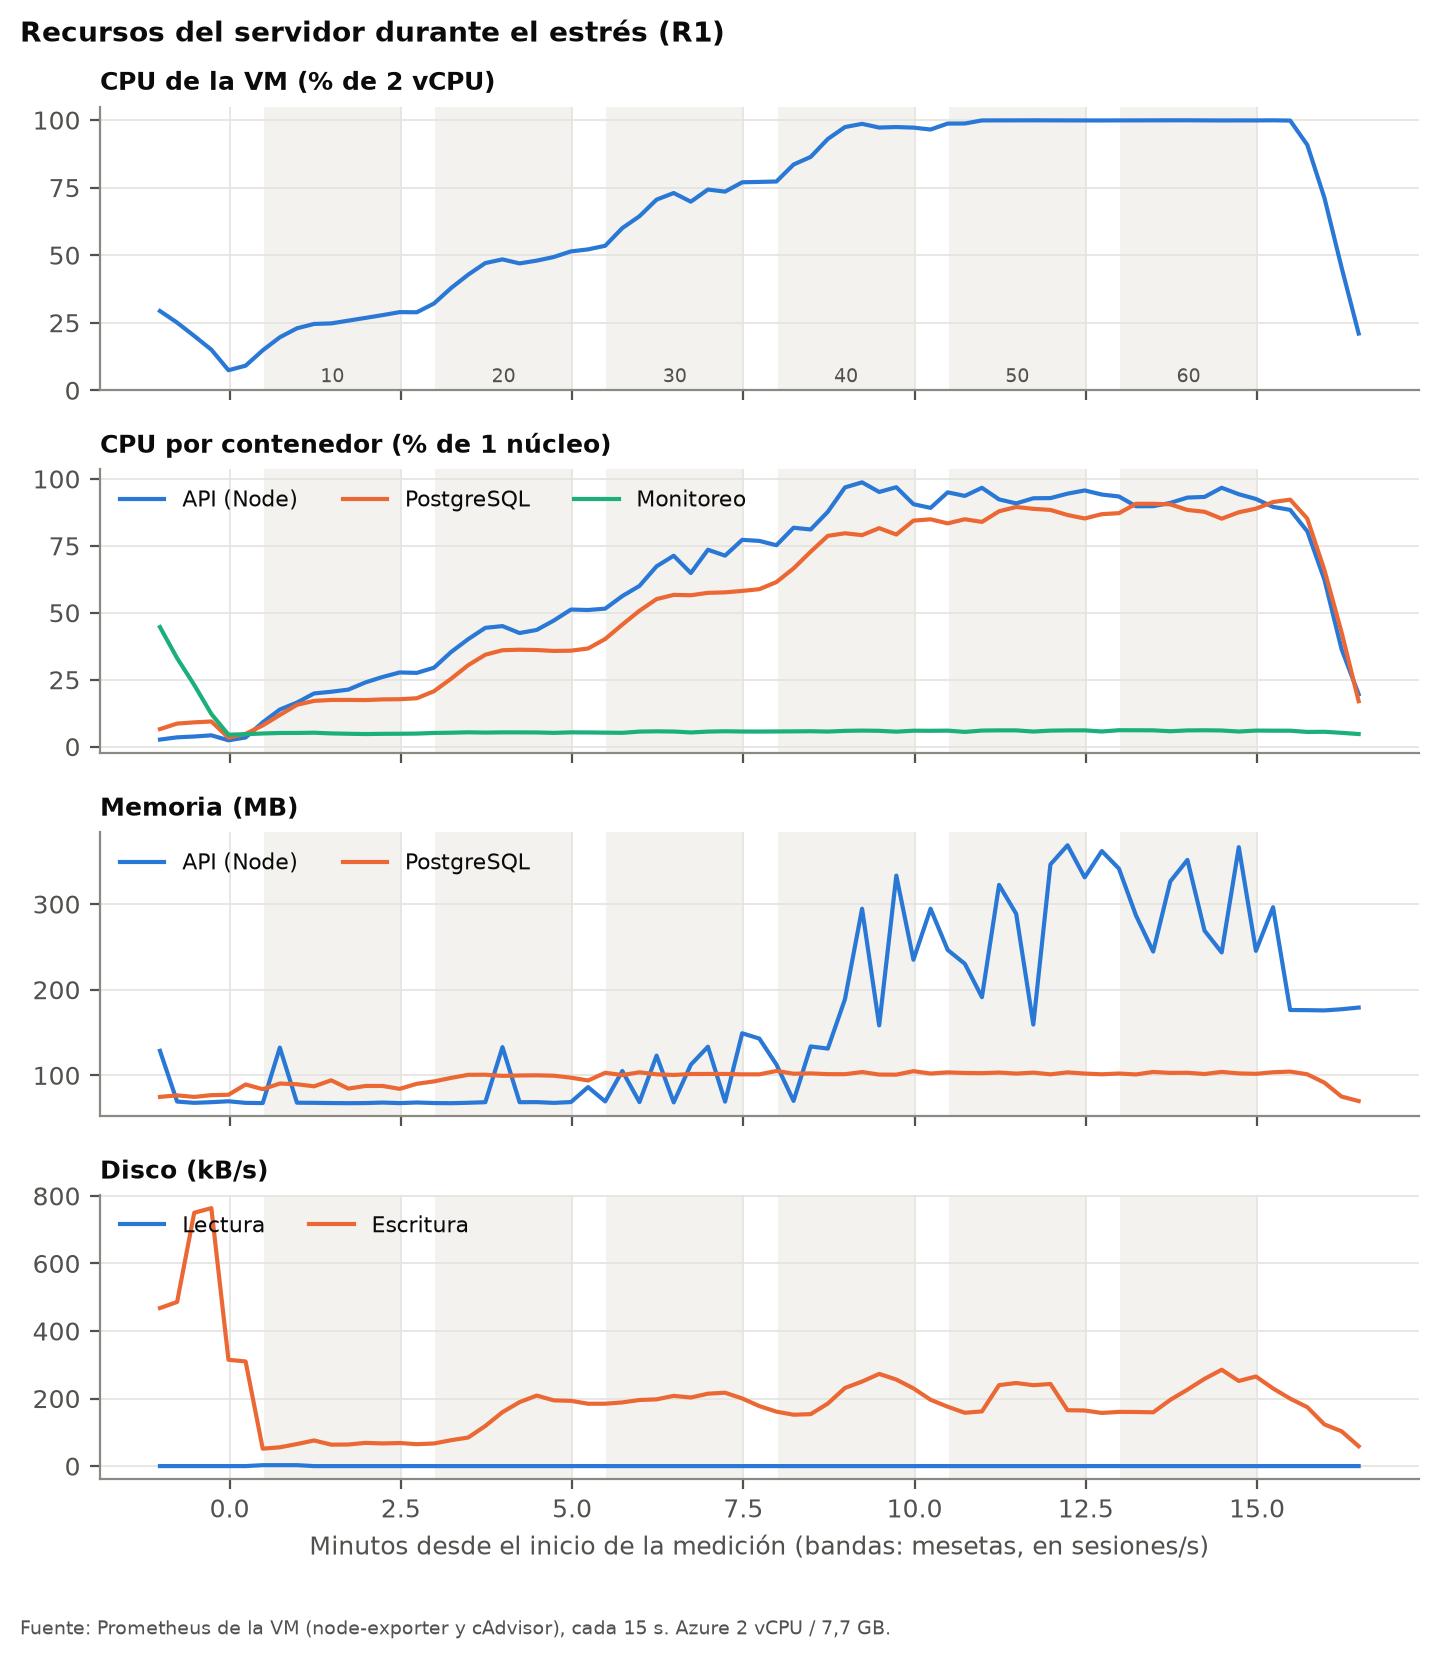
\includegraphics[height=5.3cm]{06_recursos_servidor_estres.png}
    \end{column}
    \begin{column}{0.44\textwidth}
      \small
      \begin{itemize}
        \item CPU 95 \% en 40 ses/s, 100 \% desde 50
        \item API $\approx$ 94 \% y PostgreSQL $\approx$ 86 \% de un núcleo
        \item Memoria y disco lejos del límite
        \item Ley de utilización: $X_{\max} \approx 41$ ses/s (medido 40--45)
      \end{itemize}
    \end{column}
  \end{columns}
\end{frame}

\begin{frame}{Experiencia de usuario: sin carga vs. bajo carga}
  \vspace{0.7cm}
  \begin{columns}[T]
    \begin{column}{0.64\textwidth}
      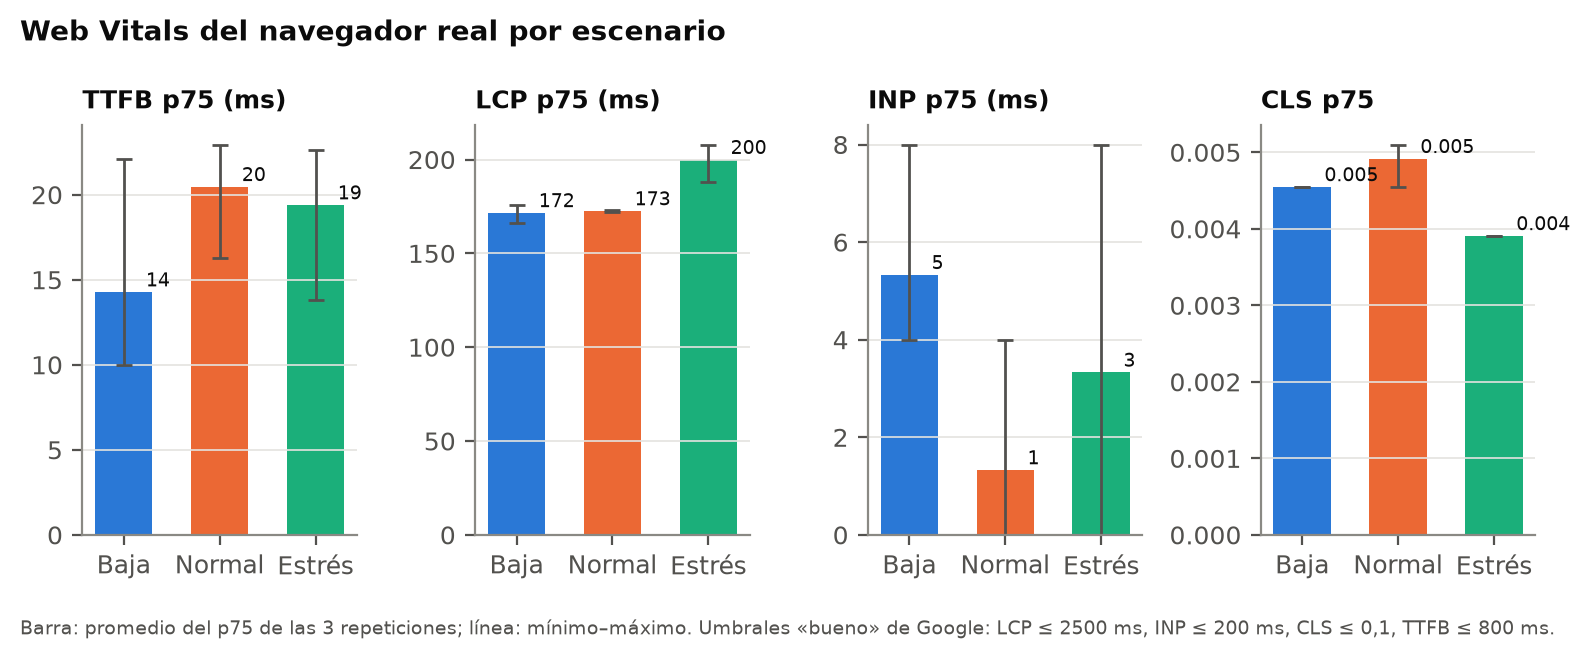
\includegraphics[width=\linewidth]{09_web_vitals_escenarios.png}
    \end{column}
    \begin{column}{0.32\textwidth}
      \small
      \begin{itemize}
        \item Web Vitals «buenas»; LCP +16 \% en estrés
        \item GA4: rebote 0 \% $\rightarrow$ 1,3 \% en estrés
        \item Conversión estable ($\approx$ 9,5 \%)
      \end{itemize}
    \end{column}
  \end{columns}
\end{frame}

% -----------------------------------------------------------------------------
% Bloque 6 – Cuellos de botella, mejoras y conclusiones
\begin{frame}{Cuello de botella y mejoras}
  \vspace{0.6cm}
  \begin{columns}[T]
    \begin{column}{0.55\textwidth}
      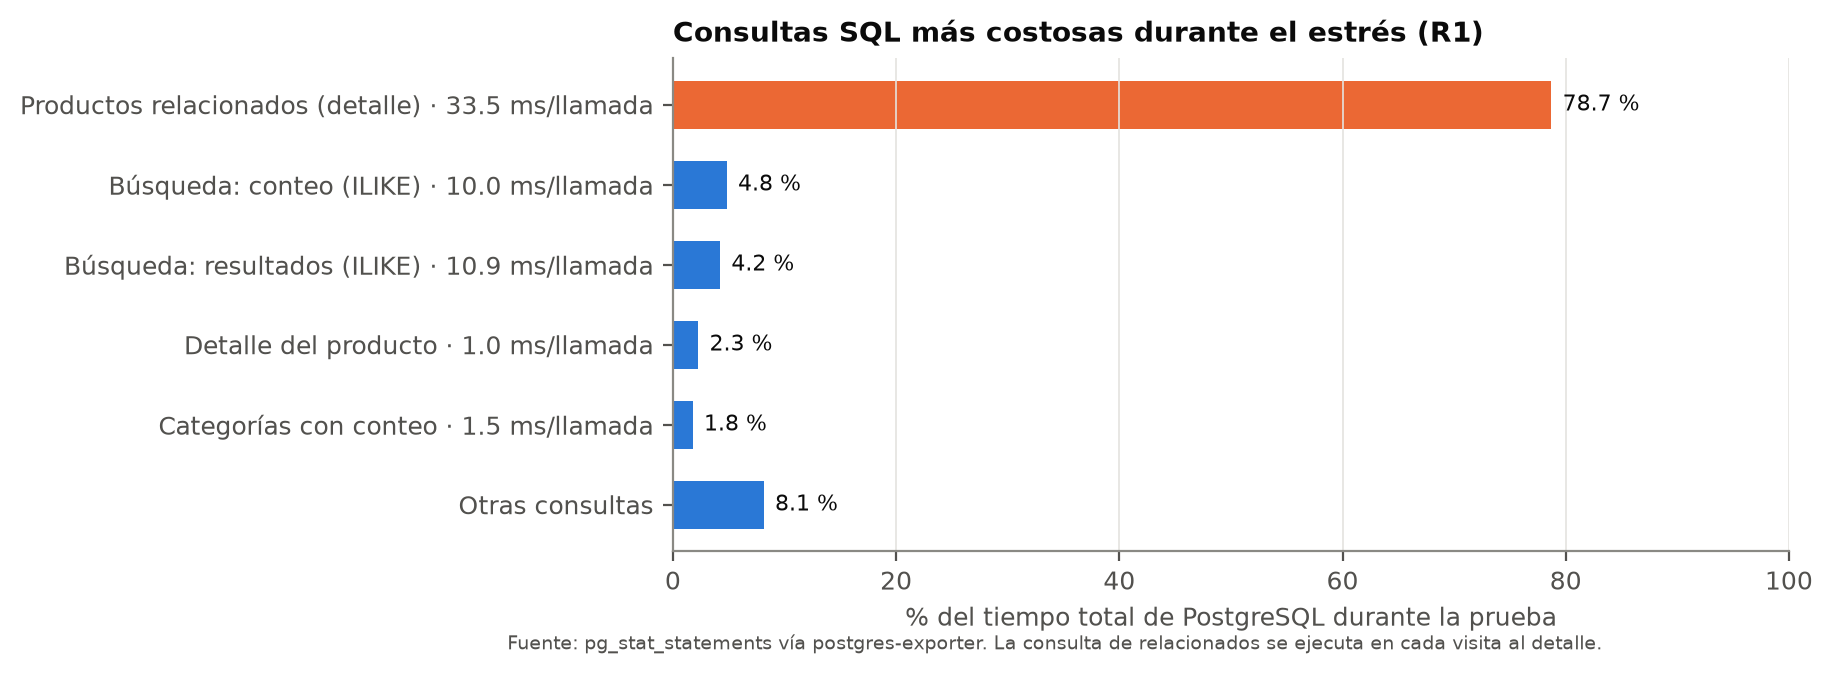
\includegraphics[width=\linewidth]{10_consultas_sql_estres.png}
    \end{column}
    \begin{column}{0.42\textwidth}
      \small
      \textbf{Una consulta = 79 \% de PostgreSQL}: «relacionados» suma todas las ventas en cada visita.
      \begin{enumerate}
        \item Precalcular ventas o caché
        \item Más CPU o base aparte
        \item Índice trigram en búsqueda
      \end{enumerate}
    \end{column}
  \end{columns}
\end{frame}

\begin{frame}{Conclusiones}
  \vspace{0.6cm}
  \izq{\begin{itemize}
    \item Carga baja y normal: SLO cumplidos con holgura (p95 $<$ 20 ms)
    \item Capacidad actual: \textbf{$\sim$40 sesiones/s ($\sim$155 req/s)}
    \item Límite: la \textbf{CPU} de la VM; una consulta domina la base de datos
    \item La ley de utilización predijo la capacidad con $<$ 10 \% de error
    \item Medir cliente y servidor a la vez evitó culpar al servidor por errores del generador
  \end{itemize}}
\end{frame}

% -----------------------------------------------------------------------------
\begin{frame}[plain]
  \begin{center}
    \vspace{0.8cm}
    
\includegraphics[height=1.6cm]{logo-utem.png}\\[0.5cm]
    {\color{verdeutem}\rule{0.6\paperwidth}{1.5pt}}\\[0.4cm]
    {\LARGE\bfseries\color{azulutem} Gracias}\\[0.3cm]
    \small Repositorio: \texttt{github.com/Wlvdi/trabajo-desempeno}\\
    Sitio: \texttt{subligol-utem.chilecentral.cloudapp.azure.com}
  \end{center}
\end{frame}

\end{document}
